\chapter{Analítica serverless}
Analytics se implementó como una API FastAPI que delega consultas en Amazon Athena. Su cliente inicia una ejecución, realiza \textit{polling} hasta \texttt{SUCCEEDED}, \texttt{FAILED} o \texttt{CANCELLED}, y devuelve las filas como JSON. La ubicación de resultados se configura mediante \texttt{ATHENA\_OUTPUT\_BUCKET}.

Los datos operacionales de ASTRA CLOUD pertenecen a dominios diferentes: el catálogo se almacena en PostgreSQL, la información social en MySQL y las interacciones en MongoDB. Los contenedores de ingesta los extraen en archivos CSV y los depositan en Amazon S3; AWS Glue permite catalogar esas estructuras y Athena ejecuta SQL sobre la información consolidada. De esta manera se desarrollaron análisis transversales sin trasladar carga de consulta a los microservicios transaccionales.

\section{Consultas analíticas en AWS Athena}
\lstset{language=SQL,basicstyle=\ttfamily\scriptsize,breaklines=true,frame=single,framesep=5pt,backgroundcolor=\color{black!3},keywordstyle=\color{utecblue}\bfseries,commentstyle=\color{gray}\itshape,captionpos=b}

\subsection*{Consulta 1: Engagement por género}
Para analizar el nivel de participación por categoría cinematográfica se desarrolló la siguiente consulta. Integra \texttt{genre}, \texttt{movie\_genre}, \texttt{movie}, \texttt{watch\_rooms} e \texttt{iteraction}; así obtiene el total de películas, salas de visualización, rating promedio, reseñas y likes para cada género.

\begin{lstlisting}[caption={Consulta SQL de engagement por género en Athena},label={lst:athena-engagement-genero}]
WITH movie_stats AS (
    SELECT m.id as movie_id, m.rating as avg_rating,
        (SELECT COUNT(DISTINCT id)
         FROM "astra_analytics"."watch_rooms"
         WHERE movie_id = CAST(m.public_id AS VARCHAR)) as watch_rooms,
        (SELECT COUNT(1) FROM "astra_analytics"."iteraction"
         WHERE movie_id = CAST(m.public_id AS VARCHAR)
           AND partition_0 = 'reviews') as total_reviews,
        (SELECT COUNT(1) FROM "astra_analytics"."iteraction"
         WHERE movie_id = CAST(m.public_id AS VARCHAR)
           AND partition_0 = 'likes') as total_likes
    FROM "astra_analytics"."movie" m
)
SELECT g.name as genre_name, COUNT(DISTINCT mg.movie_id) as total_movies,
    SUM(ms.watch_rooms) as total_watch_rooms,
    AVG(ms.avg_rating) as avg_rating, SUM(ms.total_reviews) as total_reviews,
    SUM(ms.total_likes) as total_likes
FROM "astra_analytics"."genre" g
JOIN "astra_analytics"."movie_genre" mg ON g.id = mg.genre_id
JOIN movie_stats ms ON mg.movie_id = ms.movie_id
GROUP BY g.name
ORDER BY total_watch_rooms DESC;
\end{lstlisting}

El CTE \texttt{movie\_stats} calcula las métricas por película antes de agruparlas por género. Las subconsultas relacionan el identificador público del catálogo con los registros consolidados de salas e interacciones, mientras que la consulta exterior suma y promedia los indicadores por categoría.

La Figura~\ref{fig:athena-engagement-genero} presenta la ejecución completada en Athena. En las filas visibles, Drama concentra 8\,567 \textit{watch rooms}, 8\,495 reseñas y 10\,651 likes; Comedy aparece a continuación con 6\,549 salas. Estos resultados permiten priorizar el análisis de actividad de las categorías con mayor participación.

\begin{figure}[H]
  \centering
  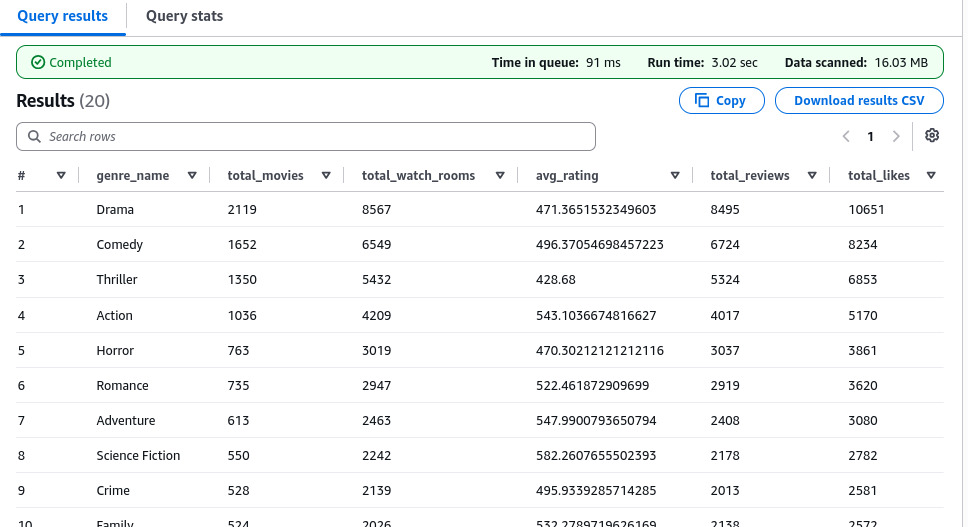
\includegraphics[width=.96\textwidth]{evidence/athena-consulta1-engagement-genero.jpeg}
  \caption{Resultado de la consulta de engagement por género en AWS Athena}
  \label{fig:athena-engagement-genero}
\end{figure}

\clearpage
\subsection*{Consulta 2: Participación de usuarios en la plataforma}
Para obtener una visión consolidada de participación se desarrolló una consulta que compara la población registrada con los usuarios únicos que intervienen en clubes, \textit{watch rooms} y reseñas. Se utilizan las tablas \texttt{users}, \texttt{memberships}, \texttt{watch\_participants} e \texttt{iteraction}. \texttt{COUNT(1)} mide el total registrado, mientras que \texttt{COUNT(DISTINCT ...)} evita contar más de una vez a un usuario que participa repetidamente en una funcionalidad.

\begin{lstlisting}[caption={Consulta SQL de participación de usuarios en Athena},label={lst:athena-participacion-usuarios}]
SELECT
    (SELECT COUNT(1) FROM "astra_analytics"."users") AS registered_users,
    (SELECT COUNT(DISTINCT user_id)
     FROM "astra_analytics"."memberships") AS users_in_clubs,
    (SELECT COUNT(DISTINCT user_id)
     FROM "astra_analytics"."watch_participants") AS users_in_watch_rooms,
    (SELECT COUNT(DISTINCT user_id)
     FROM "astra_analytics"."iteraction"
     WHERE partition_0 = 'reviews') AS reviewers;
\end{lstlisting}

La consulta concentra cuatro agregaciones independientes en una única fila de resultado. Esta forma de presentación facilita la comparación de la base de usuarios con su participación en las funcionalidades sociales de ASTRA CLOUD.

Como se aprecia en la Figura~\ref{fig:athena-participacion-usuarios}, Athena devuelve 50\,000 usuarios registrados, 47\,595 usuarios en clubes, 37\,612 participantes en \textit{watch rooms} y 16\,541 revisores. La consulta proporciona una referencia directa de la presencia de usuarios en cada etapa considerada.

\begin{figure}[H]
  \centering
  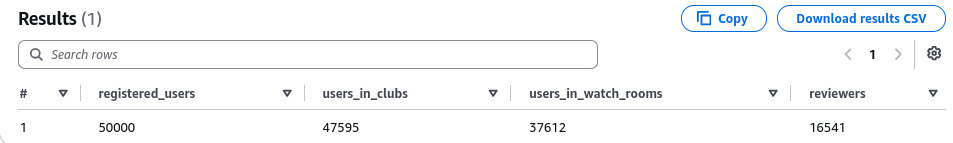
\includegraphics[width=.94\textwidth]{evidence/athena-consulta2-participacion-usuarios.jpeg}
  \caption{Resultado de la consulta de participación de usuarios en AWS Athena}
  \label{fig:athena-participacion-usuarios}
\end{figure}

\subsection*{Consulta 3: Métricas de interacción por película}
Para integrar el catálogo con las interacciones y las salas de visualización se construyó una consulta analítica por película. Participan \texttt{movie}, \texttt{iteraction} y \texttt{watch\_rooms}; el resultado incluye identificador público, título, rating de catálogo, promedio de puntuaciones de usuarios, likes y cantidad de salas asociadas.

\begin{lstlisting}[caption={Consulta SQL de métricas de interacción por película en Athena},label={lst:athena-metricas-peliculas}]
WITH movie_metrics AS (
    SELECT m.public_id, m.title, m.rating AS catalog_rating,
        (SELECT AVG(CAST(score AS DOUBLE))
         FROM "astra_analytics"."iteraction"
         WHERE movie_id = CAST(m.public_id AS VARCHAR)
           AND partition_0 = 'reviews') AS avg_user_review_score,
        (SELECT COUNT(1) FROM "astra_analytics"."iteraction"
         WHERE movie_id = CAST(m.public_id AS VARCHAR)
           AND partition_0 = 'likes') AS likes_count,
        (SELECT COUNT(1) FROM "astra_analytics"."watch_rooms"
         WHERE movie_id = CAST(m.public_id AS VARCHAR)) AS watch_room_count
    FROM "astra_analytics"."movie" m
)
SELECT * FROM movie_metrics
ORDER BY watch_room_count DESC
LIMIT 100;
\end{lstlisting}

El CTE \texttt{movie\_metrics} construye primero los indicadores por película. Posteriormente, Athena ordena las filas por \texttt{watch\_room\_count} de forma descendente y limita la salida a las primeras 100 películas, manteniendo una vista manejable para el consumo de la API analítica.

La Figura~\ref{fig:athena-metricas-peliculas} registra una ejecución completada con 100 resultados. La captura muestra, entre las primeras filas, títulos como \textit{Contracted: Phase II}, \textit{Getting Even with Dad} y \textit{Rise of the Guardians}, junto con sus identificadores públicos y los campos de métricas. Esta vista permite relacionar directamente los datos del catálogo con la actividad registrada en la plataforma.

\begin{figure}[H]
  \centering
  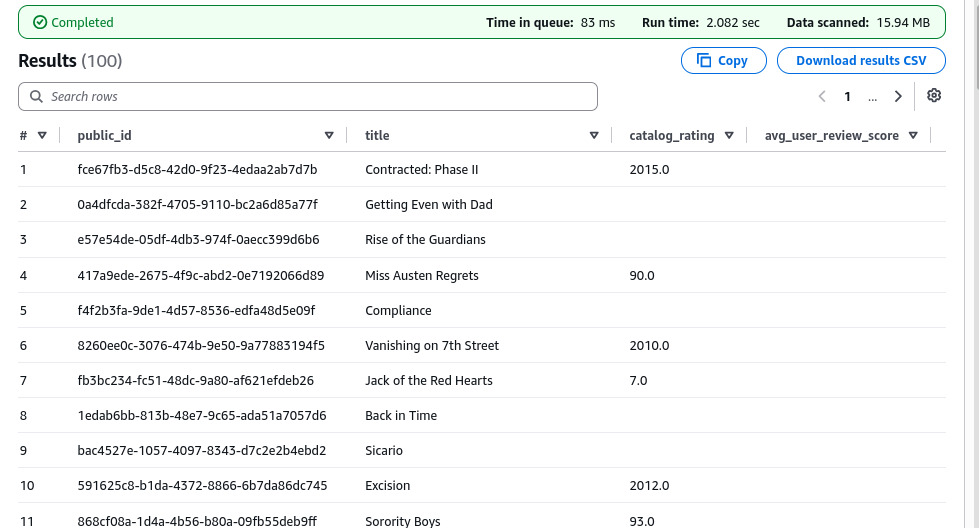
\includegraphics[width=.96\textwidth]{evidence/athena-consulta3-metricas-peliculas.jpeg}
  \caption{Resultado de la consulta de métricas de interacción por película en AWS Athena}
  \label{fig:athena-metricas-peliculas}
\end{figure}

\subsection*{Consulta 4: Nivel de actividad de los clubes}
Para analizar la actividad de las comunidades de ASTRA CLOUD se desarrolló una consulta que relaciona los clubes con sus miembros, las salas creadas y la diversidad de películas visualizadas. Participan las tablas \texttt{clubs}, \texttt{memberships} y \texttt{watch\_rooms}; el resultado incluye el nombre del club, miembros únicos, salas, relación de actividad y películas diferentes asociadas.

\begin{lstlisting}[caption={Consulta SQL de nivel de actividad de clubes en Athena},label={lst:athena-actividad-clubes}]
SELECT c.name AS club_name,
    COUNT(DISTINCT m.user_id) AS member_count,
    COUNT(DISTINCT wr.id) AS total_watch_rooms,
    CAST(COUNT(DISTINCT wr.id) AS DOUBLE)
        / NULLIF(COUNT(DISTINCT m.user_id), 0) AS activity_ratio,
    COUNT(DISTINCT wr.movie_id) AS unique_movies_watched
FROM "astra_analytics"."clubs" c
LEFT JOIN "astra_analytics"."memberships" m ON c.id = m.club_id
LEFT JOIN "astra_analytics"."watch_rooms" wr ON c.id = wr.club_id
GROUP BY c.name
ORDER BY activity_ratio DESC NULLS LAST;
\end{lstlisting}

Los \texttt{LEFT JOIN} conservan los clubes aunque todavía no tengan membresías o salas asociadas. A su vez, \texttt{NULLIF} evita una división entre cero cuando un club no registra miembros; esto permite ordenar la actividad sin excluir comunidades de la visión analítica.

La Figura~\ref{fig:athena-actividad-clubes} muestra 1\,712 resultados ordenados por \texttt{activity\_ratio}. En las filas visibles, Townsend-Wood Club 1456 registra 53 miembros, 11 salas y una relación de actividad de aproximadamente 0.208; Huerta-Wallace Club 307 registra 79 miembros y 13 salas. La consulta permite comparar la creación de salas con el tamaño de cada comunidad.

\begin{figure}[H]
  \centering
  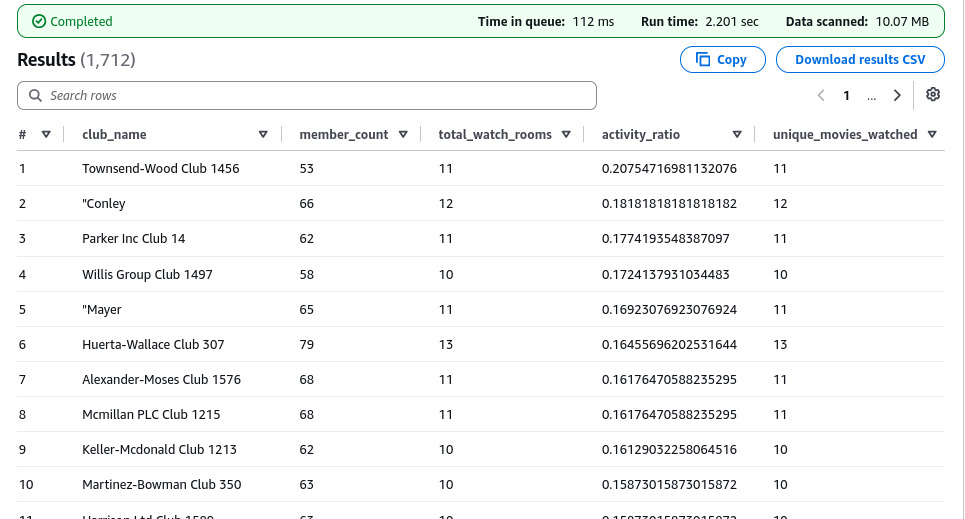
\includegraphics[width=.96\textwidth]{evidence/athena-consulta4-actividad-clubes.jpeg}
  \caption{Resultado de la consulta de actividad de clubes en AWS Athena}
  \label{fig:athena-actividad-clubes}
\end{figure}

\section{Vistas analíticas en AWS Athena}
Además de las consultas analíticas, se implementaron vistas en Athena para encapsular integraciones que se reutilizan dentro de ASTRA CLOUD. Cada vista reúne en una estructura consultable los datos que originalmente pertenecen a distintos componentes de la plataforma.

\subsection*{Vista 1: Consolidado analítico de películas}
La vista \texttt{vw\_consolidado\_peliculas} crea una representación reutilizable del catálogo, sus géneros, las salas de visualización y las interacciones. Proporciona identificador de película, título, género, total de salas, total de likes y promedio de puntuaciones de usuarios a partir de \texttt{movie}, \texttt{movie\_genre}, \texttt{genre}, \texttt{watch\_rooms} e \texttt{iteraction}.

\begin{lstlisting}[caption={Creación de la vista vw\_consolidado\_peliculas},label={lst:athena-vista-consolidado}]
CREATE OR REPLACE VIEW vw_consolidado_peliculas AS
SELECT m.public_id AS movie_id, m.title, g.name AS genre,
    COUNT(DISTINCT w.id) AS total_salas,
    COUNT(i_likes.user_id) AS total_likes,
    AVG(CAST(i_reviews.score AS DOUBLE)) AS promedio_usuarios
FROM "astra_analytics"."movie" m
LEFT JOIN "astra_analytics"."movie_genre" mg ON m.id = mg.movie_id
LEFT JOIN "astra_analytics"."genre" g ON mg.genre_id = g.id
LEFT JOIN "astra_analytics"."watch_rooms" w
    ON CAST(m.public_id AS VARCHAR) = w.movie_id
LEFT JOIN "astra_analytics"."iteraction" i_likes
    ON CAST(m.public_id AS VARCHAR) = i_likes.movie_id
    AND i_likes.partition_0 = 'likes'
LEFT JOIN "astra_analytics"."iteraction" i_reviews
    ON CAST(m.public_id AS VARCHAR) = i_reviews.movie_id
    AND i_reviews.partition_0 = 'reviews'
GROUP BY m.public_id, m.title, g.name;
\end{lstlisting}

La Figura~\ref{fig:athena-vista1-creacion} registra la creación exitosa de la vista y la Figura~\ref{fig:athena-vista1-consulta} presenta su consulta. En las filas visibles aparecen \textit{Jurassic World}, \textit{Mad Max: Fury Road} y \textit{Terminator Genisys}, con sus géneros, salas y likes consolidados. La vista evita reconstruir manualmente estas relaciones en cada análisis posterior.

\begin{figure}[H]
  \centering
  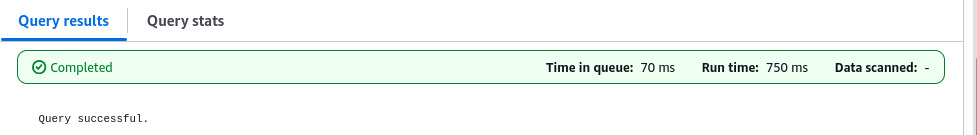
\includegraphics[width=.76\textwidth]{evidence/athena-vista1-creacion.jpeg}
  \caption{Creación de la vista vw\_consolidado\_peliculas en AWS Athena}
  \label{fig:athena-vista1-creacion}
\end{figure}
\begin{figure}[H]
  \centering
  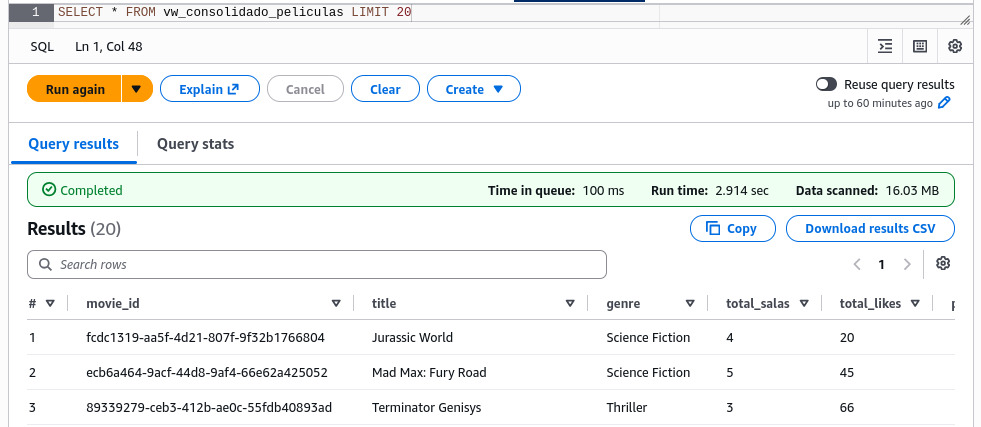
\includegraphics[width=.96\textwidth]{evidence/athena-vista1-consulta.jpeg}
  \caption{Consulta de la vista vw\_consolidado\_peliculas en AWS Athena}
  \label{fig:athena-vista1-consulta}
\end{figure}

\subsection*{Vista 2: Perfil social de usuarios}
La vista \texttt{vw\_perfil\_social\_usuarios} consolida la participación social de cada usuario. Relaciona \texttt{users}, \texttt{memberships} y \texttt{watch\_participants} para ofrecer identificador, username, correo electrónico, clubes unidos y salas en las que participó.

\begin{lstlisting}[caption={Creación de la vista vw\_perfil\_social\_usuarios},label={lst:athena-vista-perfil}]
CREATE OR REPLACE VIEW vw_perfil_social_usuarios AS
SELECT u.id AS user_id, u.username, u.email,
    COUNT(DISTINCT m.club_id) AS clubes_unidos,
    COUNT(DISTINCT wp.watch_room_id) AS salas_participadas
FROM "astra_analytics"."users" u
LEFT JOIN "astra_analytics"."memberships" m
    ON CAST(u.id AS VARCHAR) = CAST(m.user_id AS VARCHAR)
LEFT JOIN "astra_analytics"."watch_participants" wp
    ON CAST(u.id AS VARCHAR) = CAST(wp.user_id AS VARCHAR)
GROUP BY u.id, u.username, u.email;
\end{lstlisting}

La creación de la vista se muestra en la Figura~\ref{fig:athena-vista2-creacion} y su consulta en la Figura~\ref{fig:athena-vista2-consulta}. Las filas visibles incluyen usuarios con diferentes combinaciones de clubes y salas, como \texttt{jeanmoreno\_3781} con 4 clubes y 4 salas. Esta representación resume la presencia de cada usuario en las funcionalidades sociales sin repetir los conteos en cada consulta de consumo.

\begin{figure}[H]
  \centering
  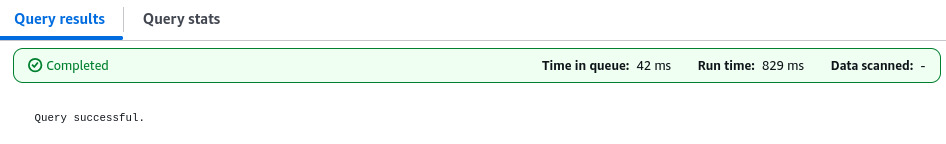
\includegraphics[width=.76\textwidth]{evidence/athena-vista2-creacion.jpeg}
  \caption{Creación de la vista vw\_perfil\_social\_usuarios en AWS Athena}
  \label{fig:athena-vista2-creacion}
\end{figure}
\begin{figure}[H]
  \centering
  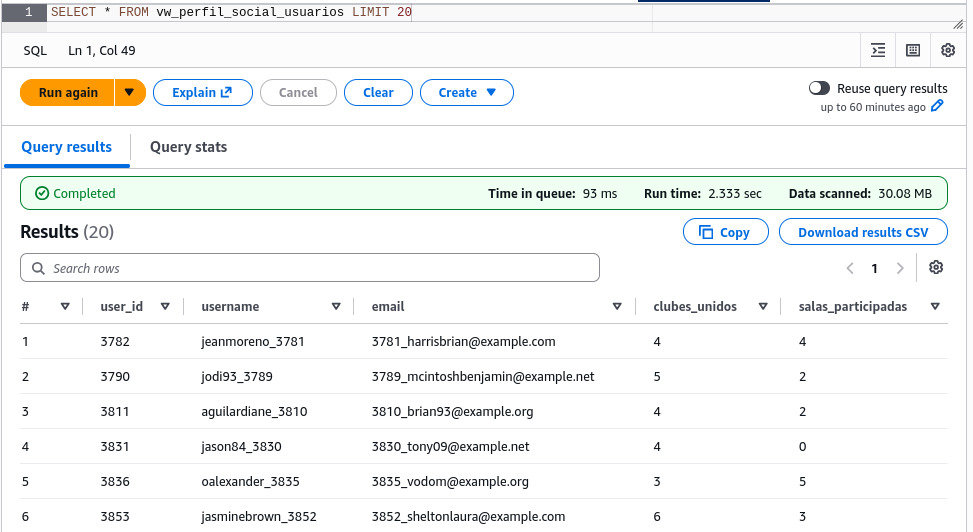
\includegraphics[width=.96\textwidth]{evidence/athena-vista2-consulta.jpeg}
  \caption{Consulta de la vista vw\_perfil\_social\_usuarios en AWS Athena}
  \label{fig:athena-vista2-consulta}
\end{figure}
